\documentclass[a4paper,12pt,reqno]{amsart}
\usepackage{M67tds}

% pour voir les solutions il faut enlever le commentaire de la ligne suivante
\solutionstrue

\newlist{axioms}{description}{1}
\newcommand\axiomlabel[1]{\hfill\textbf{(#1)}}
\setlist[axioms]{style=nextline,before={\let\makelabel\axiomlabel}}

% Les notes de bas de page dans les minipages (sidebyside)
\renewcommand{\thempfootnote}{\fnsymbol{mpfootnote}}

% pour surligner
\sisolutions{
  \usepackage{soul}
  \colorlet{hl}{yellow!35!white}
  \sethlcolor{hl}
}

\begin{document}

% ==================================
\hautdepage{

\ifsolutions{Solutions de l'interrogation}\else{Interrogation}\fi\par\normalfont\normalsize
5 mars 2018\\{[ durée: 2 heures ]}\par
}
% ==================================
\ifsolutions\else
% {\fontencoding{U}\fontfamily{futs}\selectfont\char 66\relax}
\tikz[baseline=(e.base)]{\NoAutoSpacing\node(e){!};\draw[red,ultra thick,line join=round,yshift=-.15ex](90:1em)--(210:1em)--(330:1em)--cycle;}
\textbf{Documents autorisés :}\textit{Une feuille A4 recto-verso écrite à la main.}

\vspace{7mm}
\tsvp
\fi

%-----------------------------------
\begin{exo} (Construction à la règle et compas)

  Soient $O(0,0)$ et $I(1,0)$ deux points donnés du plan euclidien. Illustrer par un dessin et donner un programme de construction à la règle et au compas à partir de $O$ et $I$:
  \begin{enumerate}
    \item du point $J(0,1)$,
    \item du point $K(\frac23,0)$,
    \item de points $L \in [O,I)$ et $M$ tels que $\tri OLM$ soit rectangle en $M$, $OL=\frac43$ et $LM=\frac23$.
  \end{enumerate}
\end{exo}

\begin{solution}

  \begin{convention}
    On note $C(X,Y)$ le cercle de centre $X$ passant par $Y$, $C(X,YZ)$ le cercle de centre X et de rayon $YZ$ (qui est constructible si $X$, $Y$ et $Z$ le sont) et $C^{*}(X,Y) = C(X,Y)\setminus\{Y\}$.
  \end{convention}
  \sidebyside{.70}{
    \begin{enumerate}
      \item
      \begin{itemize}
        \item Soit $A = (OI)\cap C^{*}(O,I)$;
        \item on construit la médiatrice de $[AI]$ passant par $C(A,I)\cap C(I,A)$;
        \item alors $J \in \text{médiatrice de }[AI] \cap C(O,I)$.
      \end{itemize}
      \item
      \begin{itemize}
        \item Soit $B = (OJ) \cap C^{*}(J,O)$;
        \item soit $C = (OJ) \cap C^{*}(B,J)$;
        \item on considère la droite passant par $B$ parallèle à $(CI)$, qui passe par $C(I,CB)\cap C(B,CI)$, et qui coupe $(OI)$ en $K$. En effet par Thalès $OK:OI = OB:OC = 2:3$.
      \end{itemize}
    \end{enumerate}
  }{
    \raisebox{-17mm}[5cm][0pt]{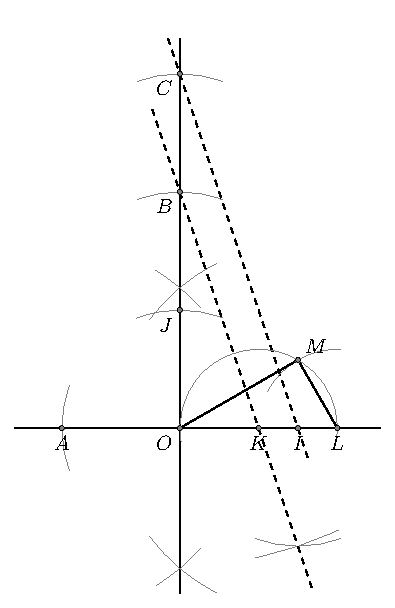
\includegraphics[width=47mm]{M67_2017-18_DS1_img_construction1}}
  }\vskip 3pt
  \begin{enumerate}\setcounter{enumi}{2}
    \item
    \begin{itemize}
      \item Soit $L = C^{*}(K,O) \cap (OI)$;
      \item soit $M = C^{*}(K,O) \cap C^{*}(L,K)$. En effet comme $M$ est sur le cercle de diamètre $OL$ le triangle est rectangle en $M$ et $LM=LK=\frac{2}{3}$ par construction.
    \end{itemize}
  \end{enumerate}
  \newpage % bidouillage sur la mise en page
\end{solution}

%-----------------------------------
\begin{exo} (Axiomatique)

  On rappelle les propriétés d'incidence et d'ordre:\\[-1.7\baselineskip]
  \begin{multicols}{2}\small
    \begin{axioms}[leftmargin=3.5em]
      \item[I1] par deux points distincts passe une unique droite,
      \item[I2] toute droite contient au moins deux points distincts,
      \item[I3] il existe trois points non alignés,
      \item[O1] si $C$ est entre $A$ et $B$, alors $A$, $B$ et $C$ sont alignés, deux à deux distincts et $C$ est aussi entre $B$ et $A$,
      \item[O2] pour tous points distincts $A$ et $B$ il existe un point $C$ tel que $B$ soit entre $A$ et $C$,
      \item[O3] parmi trois points alignés deux à deux distincts, un et un seul d'entre eux est entre les deux autres,
      \item[O4] soient $A$, $B$, et $C$ trois points non alignés et $\ens{D}$ une droite ne passant par aucun d'eux. Si $\ens{D}$ passe par un point $D$ entre $A$ et $B$, alors $\ens{D}$ passe ou bien par un point entre $A$ et $C$, ou bien par un point entre $B$ et $C$, mais pas les deux à la fois.
    \end{axioms}
  \end{multicols}\vspace{7pt}
  \sidebyside{.7}{
    En utilisant seulement les propriétés \textbf{I1} à \textbf{O4} démontrer que si deux points distincts $C$ et $D$ sont entre $A$ et $B$ alors soit $D$ est entre $A$ et $C$,  soit $D$ est entre $B$ et $C$.\\
    \begin{indication}
      Vous pouvez vous inspirer du dessin ci-contre.
    \end{indication}
  }{
      \raisebox{-21mm}[0pt][0pt]{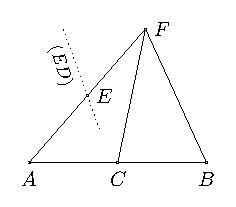
\includegraphics[width=5cm]{M67_2017-18_DS1_img_ordre}}
  }
\end{exo}

\begin{solution}

  \begin{convention}
    On note $X \in ]YZ[$ (resp. $X \notin ]YZ[$) pour désigner que $X$ \textbf{est} (resp. \textbf{n'est pas}) entre $Y$ et $Z$.
  \end{convention}

  Soit $E$ non aligné avec $A$ et $B$ \textbf{(I3)} et $F$ tel que $E \in ]AF[$ \textbf{(O2)}. Le point $F$ n'est pas aligné avec $A$ et $B$ car sinon $E$ serait sur la droite $(AF)\overset{\tiny\textbf{(I1)}}{=}(AB)$. Comme $D\neq C$ la droite $(ED)$ ne passe pas par $C$, sinon on aurait eu $(ED)\overset{\tiny\textbf{(I1)}}{=}(CD)\overset{\tiny\textbf{(I1+O1)}}{=}(AB)$, ce qui est en contradiction avec $E \notin (AB)$. Par le même type de raisonnement on obtient que $(ED)$ ne passe pas par $A$, $B$ et $F$.

  On applique \textbf{(O4)} à la droite $ED$ et aux trois points non alignés $A$, $C$ et $F$ :
  \begin{enumerate}
    \item soit $(ED)$ coupe $]AC[$ en $D$ et la question est réglée;
    \item soit $(ED)$ coupe $]FC[$.
    \begin{itemize}
      \item Dans le deuxième cas on applique d'abord \textbf{(O4)} à la droite $ED$ et aux trois points non alignés $F$, $A$ et $B$ pour conclure que $(ED)$ ne coupe pas $]FB[$ car elle coupe $]AF[$ en $E$ et $]AB[$ en $D$.
      \item Puis, on applique encore une fois \textbf{(O4)} à la droite $(ED)$ et aux trois autres points non alignés $F$, $C$ et $B$, ce qui nous permet de conclure que $D = (ED)\cap(AB) \in ]CB[$.
    \end{itemize}
  \end{enumerate}
\end{solution}


%-----------------------------------
\begin{exo} (Exemple de droite d'Euler)

  On munit le plan $\mathcal{P}$ d'un repère cartésien orthonormal et on considère les points $A$, $B$ et $C$ de coordonnées respectives $(1, 1)$, $(3, 7)$ et $(−1, 3)$.
  \begin{enumerate}
    \item
      \begin{enumerate}
        \item Déterminer une équation cartésienne de chacune des trois médianes du triangle $\tri ABC$.
        \item Vérifier que $G$ isobarycentre de $A$, $B$ et $C$ est l'intersection de ces médianes.
      \end{enumerate}
    \item
      \begin{enumerate}
        \item Déterminer une équation cartésienne de chacune des trois médiatrices du triangle $\tri ABC$.
        \item Vérifier que ces trois médiatrices sont concourantes en un point noté $O$.
      \end{enumerate}
    \item
      \begin{enumerate}
        \item Déterminer une équation cartésienne de chacune des trois hauteurs du triangle $\tri ABC$.
        \item Vérifier que ces trois hauteurs sont concourantes en un point noté $H$.
      \end{enumerate}
    \item Vérifier que les points $G$, $O$ et $H$ sont alignés.
  \end{enumerate}

\end{exo}

\begin{solution}

  \begin{enumerate}
    \item
      \begin{enumerate}
        \item \hl{La médiane issue de $A(1,1)$} passe par le milieu $(1,5)$ de $[BC]$. Ainsi son équation est \hl{$x=1$}.\\
        \hl{La médiane issue de $B(3,7)$} passe par le milieu $(0,2)$ de $[AC]$. Donc $(3,5)$ est un vecteur directeur et $(5,-3)$ est un vecteur normal. Ainsi son équation est \hl{$5x-3y=$}$5.0-3.2=$\hl{$-6$}.\\
        \hl{La médiane issue de $C(-1,3)$} passe par le milieu $(2,4)$ de $[AB]$. Donc $(3,1)$ est un vecteur directeur et $(1,-3)$ est un vecteur normal. Ainsi son équation est \hl{$x-3y=$}$-1-3.3=$\hl{$-10$}.
        \item Le barycentre $G$ a pour coordonnées $(\frac{1+3+(-1)}{3}, \frac{1+7+3}{3})=(1, 11/3)$ qui vérifient $1=1$, $5.1-3.\frac{11}{3}=-6$ et $1-3.\frac{11}{3}=-10$.
      \end{enumerate}
    \item
      \begin{enumerate}
        \item
        \hl{La médiatrice de $[AB]$} a pour vecteur normal $(2,6)=2(1,3)$ et passe par son milieu $(2,4)$. Ainsi son équation est \hl{$x+3y=$}$2+3.4=$\hl{$14$}.\\
        \hl{La médiatrice de $[BC]$} a pour vecteur normal $(4,4)=4(1,1)$ et passe par son milieu $(1,5)$. Ainsi son équation est \hl{$x+y=$}$1+5=$\hl{$6$}.\\
        \hl{La médiatrice de $[AC]$} a pour vecteur normal $(2,-2)=2(1,-1)$ et passe par son milieu $(0,2)$. Ainsi son équation est \hl{$x-y=$}$0-2=$\hl{$-2$}.

        \emph{
          Note : La médiatrice de deux points $(x_{1},y_{1})$ et $(x_{2},y_{2})$ a pour vecteur normal $(x_{1}-x_{2},y_{1}-y_{2})$ et passe par $(\frac{x_{1}+x_{2}}{2},\frac{y_{1}-y_{2}}{2})$. Donc elle est définie par l'équation
          \[
            (x_{1}-x_{2})x+(y_{1}-y_{2})y=\frac{x_{1}^{2}-x_{2}^{2}}{2}+\frac{y_{1}^{2}-y_{2}^{2}}{2}.
          \]
        }
        \item Soit $O(x,y)$ l'intersection des médiatrices de $[BC]$ et $[AC]$. Donc $(x,y)$ vérifie les deux équation $x+y=6$ et $x-y=-2$. Ainsi on trouve les coordonnées $O(2,4)$. Et comme $2+3.4=4$ on constate que $O$ est aussi sur la médiatrice de $[AB]$. \emph{Au passage on remarque aussi que $O(2,4)$ coïncide avec le milieu de $[AB]$ et donc le triangle $\tri ABC$ est rectangle en $C$.}
      \end{enumerate}
    \item
      \begin{enumerate}
        \item
        \hl{La hauteur issue de $A(1,1)$ }a pour vecteur normal $(4,4)=4(1,1)$. Ainsi son équation est \hl{$x+y=$}$1+1=$\hl{$2$}.\\
        \hl{La hauteur issue de $B(3,7)$ }a pour vecteur normal $(2,-2)=2(1,-1)$. Ainsi son équation est \hl{$x-y=$}$3-7=$\hl{$-4$}.\\
        \hl{La hauteur issue de $C(-1,3)$} a pour vecteur normal $(2,6)=2(1,3)$. Ainsi son équation est \hl{$x+3y=$}$-1+3.3=$\hl{$8$}.
        \item Soit $H(x,y)$ l'intersection des hauteurs issues de $A$ et $B$. Donc $(x,y)$ vérifie les deux équations $x+y=2$ et $x-y=-4$. Ainsi on trouve les coordonnées $H(-1,3)$. Et comme $-1+3.3=8$ on constate que $O$ est aussi sur la hauteur issue de $C$. \emph{On avait déjà remarqué que $\tri ABC$ est rectangle en $C$ et donc on savait que nécessairement $H=C$.}
      \end{enumerate}
    \item On a $(1,11/3) = \frac{1}{3}(-1,3) + \frac{2}{3}(2,4)$, donc comme $G=\frac{1}{3}H + \frac{2}{3}O$ les trois points sont alignés. \emph{Comme on avait remarqué que $H=C$ et $O$ est le milieu de $[AB]$ on savait que $G$ est sur la médiane $HO$. Par ailleurs la relation $G=\frac{1}{3}H + \frac{2}{3}O$ est vérifiée dans tous les triangles et la droite qui contient $H$,$G$ et $O$ est appelée \emph{droite d'Euler}.}
  \end{enumerate}

\end{solution}

%-----------------------------------
\begin{exo} (Kangourou 2008)

  \sidebyside{.7}{
    $\tri PQR$ est un triangle dont les longueurs des côtés, $PR$, $PQ$ et $QR$, sont respectivement $5$, $6$ et $3$. $T$ et $S$ sont deux points, respectivement pris sur les segments $[PR]$ et $[PQ]$, tels que la droite $(TS)$ soit tangente au cercle inscrit dans le triangle $\tri PQR$. Déterminer le périmètre du triangle $\tri PST$.

  }{
    \raisebox{-21mm}[0pt][0pt]{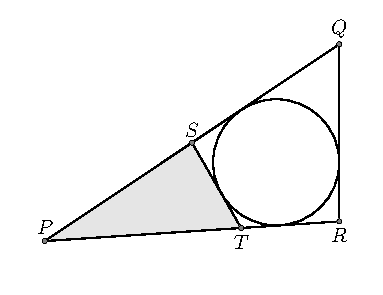
\includegraphics[width=5cm]{img_kangourou2008}}
  }
\end{exo}

\begin{solution}

  \sidebyside{.7}{
    \emph{
      On rappelle d'abord que étant donnés deux tangentes $(AB)$ et $(AC)$ issues de $A$ vers un cercle $\mathcal{C}$ (de centre $O$) avec $B,C \in \mathcal{C}$ les points de tangence, alors $AB=AC$ (par Pythagore ou par triangles égaux, car les triangles rectangles $\tri OBA$ et $\tri OCA$ ont la même hypoténuse et deux cathètes $OC=OB$ égales au rayon).
    }

  }{
    \raisebox{-21mm}[0pt][0pt]{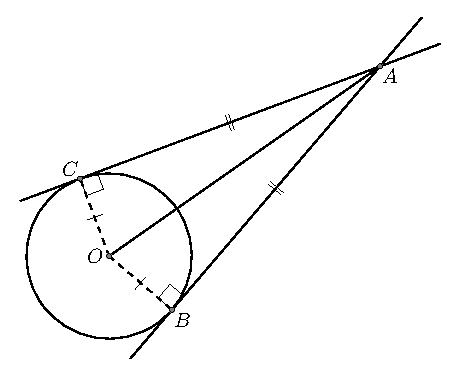
\includegraphics[width=5cm]{img_kangourou2008b}}
  }

  \sidebyside{.7}{
    Soient $U$,$V$,$W$ et $X$ les points de tangence respectivement de $(SQ)$, $(QR)$, $(RT)$ et $(TS)$. En utilisant les égalités $XS=SU$, $UQ=QV$, $VR=RW$ et $WT=TX$ on trouve pour le périmètre du triangle $\tri PST$ : $XS+SP+PT+TX=PU+PW=PQ-QU+PR-RW=PQ+PR-(QV+VR) = 5+6-3 = 8$.
  }{
    \raisebox{-21mm}[0pt][0pt]{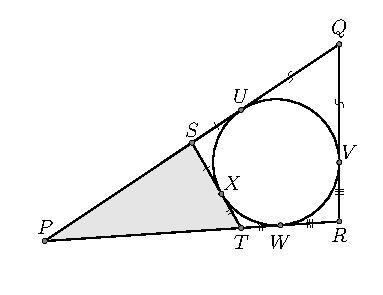
\includegraphics[width=5cm]{img_kangourou2008c}}
  }
\end{solution}


\end{document}
